
\item Two identical discs of same radius \( R \) are rotating about their axes in opposite directions with the same constant angular speed \( \omega \). The discs are in the same horizontal plane. At time \( t = 0 \), the points \( P \) and \( Q \) are facing each other as shown in the figure. The relative speed between the two points \( P \) and \( Q \) is \( v_r \). In one time period (\( T \)) of rotation of the discs, \( v_r \), as a function of time is best represented by
    \begin{center}
        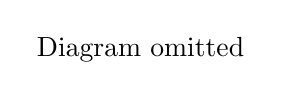
\begin{tikzpicture}
            \node at (0, 0) {Diagram omitted}; % Replace with the actual diagram if necessary
        \end{tikzpicture}
    \end{center}
    \begin{tasks}(2)
        \task \( v_r \uparrow \)
        \task \( v_r \downarrow \)
        \task \( v_r \nabla \)
        \task \( v_r \Delta \)
    \end{tasks}
